%%%%%%%%%%%%%%%%%%%%%%%%%%%%%%%%%%%%%%%%%%%%%%%%%%%%%%%%%%%%%%%%%%%%%%%%%%%
% CONTRIBUTION TO THE MESONH BOOK1: "Initial Fields for Real Flows "
% Author : S. Belair, V. Masson and F. Mereyde
% Original : September 07, 1997
% Update   : January 12, 1998
% Update   : January 17, 2000
%%%%%%%%%%%%%%%%%%%%%%%%%%%%%%%%%%%%%%%%%%%%%%%%%%%%%%%%%%%%%%%%%%%%%%%%%%%
%%%%%%%%%%%%%%%%%%%%%%%%%%%%%%%%%%%%%%%%%%%%%%%%%%%%%%%%%%%%%%%%%%%%%%%%%%%
%
\chapter{Initial Fields for Real Flows\label{REAL}}
\minitoc

%{\em by V. Masson}
%%%%%%%%%%%%%%%%%%%%%%%%%%%%%%%%%%%%%%%%%%%%%%%%%%%%%%%%%
\section{General presentation}
The simulation of realistic meteorological situations is an important scope
of Meso-NH. The preparation of initial and coupling (LB and LS) fields
by interpolation of larger-scale
meteorological analyses or forecasts, in a format ready to start a Meso-NH
experiment, is therefore an important task.
These may be produced from any situation contained in the ECMWF or Meteo-France
operational archive (including the special reanalyses projects).
A Meso-NH file, coming from a simulation at lower resolution,
can also be used as larger-scale model, to provide initial fields
- including finer surface fields and orography - for
a Meso-NH run at higher resolution
(with or without {\it gridnesting} technique).
This gives access to a wealth of possibilities.\\

\subsection{Initialization for a one-model run, from operationel models}

This type of model simulation uses one initial file (with all the fields
at beginning time of the simulation), and a certain number of coupling files
to prescribe the lateral boundary conditions to the model at further
time steps. The coupling files are of the same nature than the initial file.
Here is presented the way to produce these initial and coupling files.\\

This sequence for real cases contains three procedures or
programs (Fig. \ref{schematicsequence}).
In the following, a Fortran program is written in CAPITAL letters,
and is run with the Meso-NH procedure {\sl prepmodel} (Unix procedure
written in lower case letters).

\begin{enumerate}
\item
{PREP\_PGD}: this Meso-NH program computes the physiographic data file
(called PGD file below). At this step, you choose the projection, resolution,
and horizontal domain. The PGD file contains all the physiographic data
necessary to run the Meso-NH model with interactive surface schemes for
vegetation and town.
\item
{\sl extractecmwf}\footnote{A user is necessary on the station ecaccess of Reading to run
{\sl extractecmwf}} or {\sl extractarpege}: these two friendly procedures extract
the surface and altitude fields for one date, respectively from MARS archive
(ECMWF forecast model) or from
Meteo-France operational archive (ARPEGE and ALADIN models).
In both cases, the fields are written in a GRIB format file, on the Gaussian
grid. The extraction must be done separately for each date and time (for
the initial file and each of the coupling file).
\item
{PREP\_REAL\_CASE}: this Meso-NH program performs the change of
orography and vertical grid and writes the Meso-NH file, which will be used
either for the beginning of the simulation or for coupling.
\end{enumerate}

\subsection{Initialization for a one-model run, from a Meso-NH file}

In this case, the initial and coupling files are interpolated from a
previous Meso-NH run (at coarser resolution). It is again necessary to
produce separately one initial file and the coupling files.
The following steps are used (Fig. \ref{schematicsequence2}):
\begin{enumerate}
\item
{PREP\_PGD}
\item
{SPAWNING}: this program performs the horizontal interpolations from a
Meso-NH file into another Meso-NH file, with a finer resolution and smaller
domain.
\item
{PREP\_REAL\_CASE}
\end{enumerate}

\subsection{Initialization for a nesting run}

Two or more Meso-NH models will be run interactively. The first model, the
one with the coarser resolution and containing the others, needs again
one initial file and some coupling files (for lateral boundary conditions).

However, the nested models are contained in another Meso-NH model. This
allows to give them their lateral boundary conditions directly interpolated
from the model which contains it, at all time-steps. Therefore, no coupling file
is necessary for those models. The initial file must still be computed
before the run (the interpolation program for all the model fields is not yet
included in the model program itself).

The user can choose the date of the nested model start as he wants
(it is not necessary the same than the coarser model). The only obligation
is to start a nested model only if all the coarser models containing it
have already started, or are starting.\\

The initialisation sequence is a merging of the two previous ones
(initialisation and coupling files of the first model; initialisation
files from Meso-NH model for the nested files).  However, there is a {\bf
major change} at the beginning of the sequence: {\bf all the PGD files for
all models must be computed \underline{before} the PREP\_REAL\_CASE
program} (and as a consequence before the first model run). These PGD files
are then checked, and conformity between them for gridnesting is imposed
- the orography of one model in every grid mesh is set equal to
the average of any of its nested model orography on the same area.

The initialisation and gridnesting sequence is shown here for three models,
model~2 included in model~1, and model~3 included in model~2.
\begin{enumerate}
\item
{PREP\_PGD}: this program is run as many time as the number of models:
\begin{itemize}
\item physiographic data file for the model 1 (including projection, resolution, domain),
\item physiographic data file for the model 2 (including  resolution, domain),
\item physiographic data file for the model 3 (including  resolution, domain).
\end{itemize}
\item
{PREP\_NEST\_PGD}: this program checks all the PGD files at the same time,
and imposes the conformity between them.
\item
{\sl extractecmwf} or {\sl extractarpege}: it extracts the surface
and altitude fields for one date, for model 1.
The extraction must be done separately for each date and time (for
the initial file and each coupling file).
\item
{PREP\_REAL\_CASE}: this program is run several times, for the initial
file and the coupling files of model 1.
\item
{MESONH}: this step is {\bf optional}. If you do not wish to start
all the models at the same time, you can decide to run the model 1 before
the model 2 starts.
\item
{SPAWNING}: when you want to start the model 2, you must use this
program to compute the horizontal interpolations from the model 1 to the model
2. It is used only once.
\item
{PREP\_REAL\_CASE}: It is used only once, to compute the
initial file for the model~2. {\bf Do not change the vertical grid}.
\item
{MESONH}: again, this step is {\bf optional}. If you do not wish to start
all model 3 at the same time as model 2, you can decide to run
the models 1 and 2 alone before.
\item
{SPAWNING}: when you want to start the model 3, you must use this
program to compute the horizontal interpolations from the model 2 to the model
3. It is used only once.
\item
{PREP\_REAL\_CASE}: It is used only once, to compute the initial
file for the model~3. {\bf Do not change the vertical grid}.
\item
{MESONH}: here is now your complete nested run.
\end{enumerate}

\begin{figure}[!ht]
%\centerline{\includegraphics[width=14cm]{\EPSDIR/realcas_filiere_amont.eps}}
\centerline{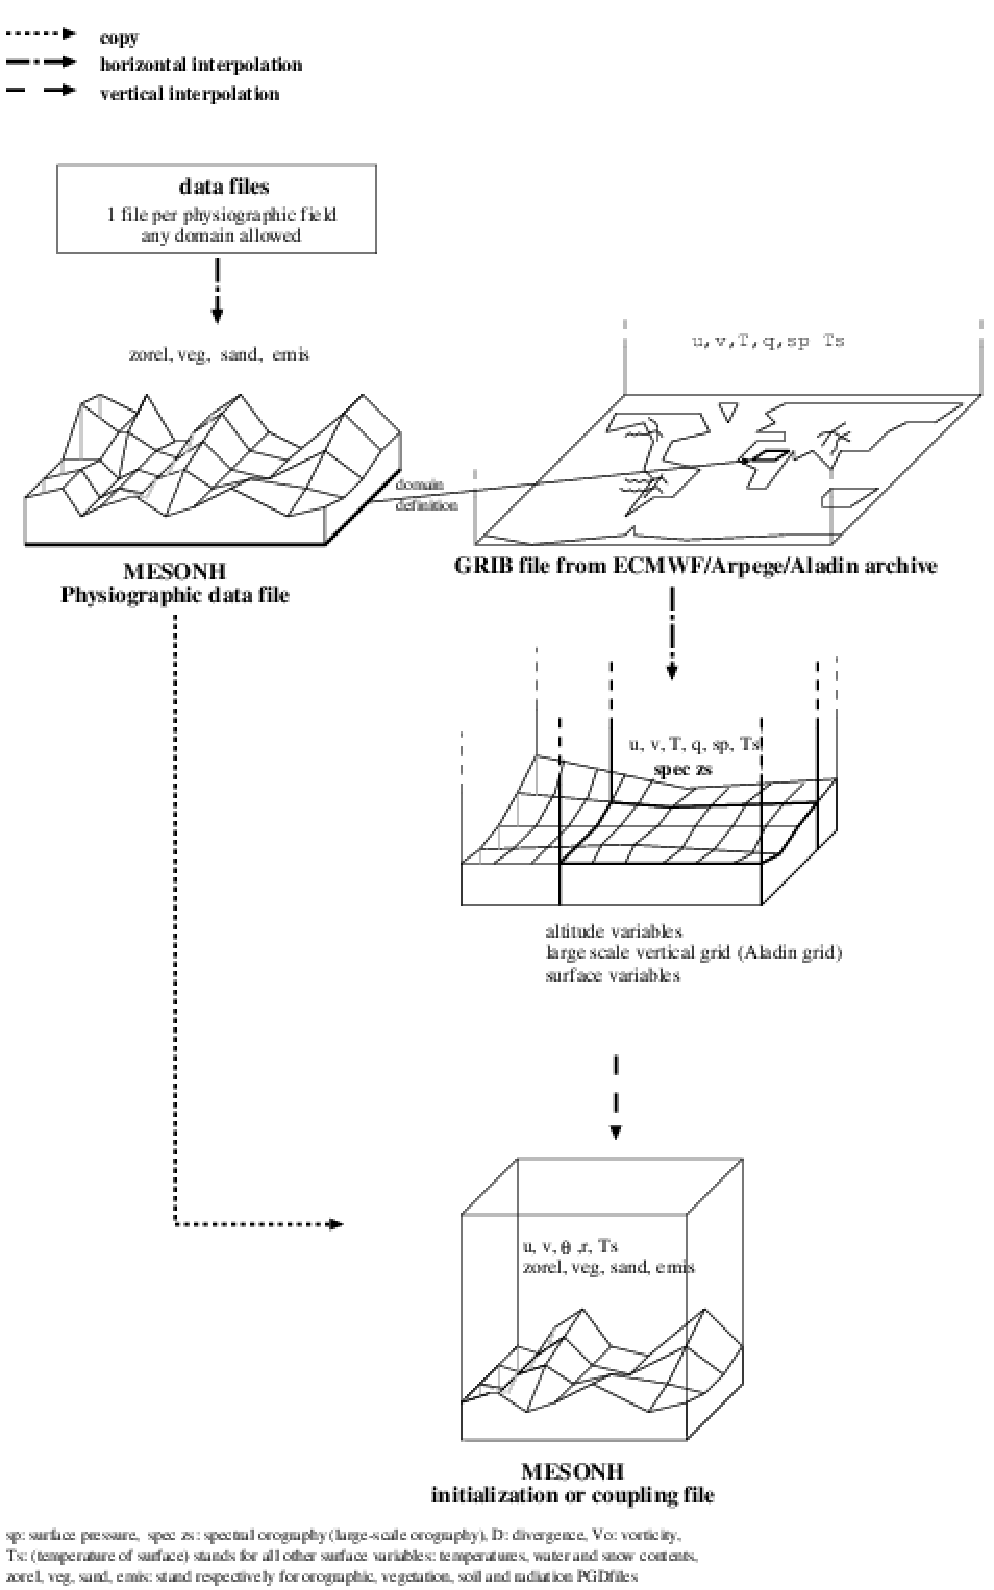
\includegraphics[width=14cm]{\EPSDIR/realcas_filiere_amont.pdf}}
\caption{schematic view of the interactions between the different files
during the initialization sequence of a real case simulation from a global file
of ECMWF or METEO-FRANCE archive.
\label{schematicsequence}}
\end{figure}

\begin{figure}[!ht]
%\centerline{\includegraphics[width=14cm]{\EPSDIR/realcas_filiere_amont_spawning.eps}}
\centerline{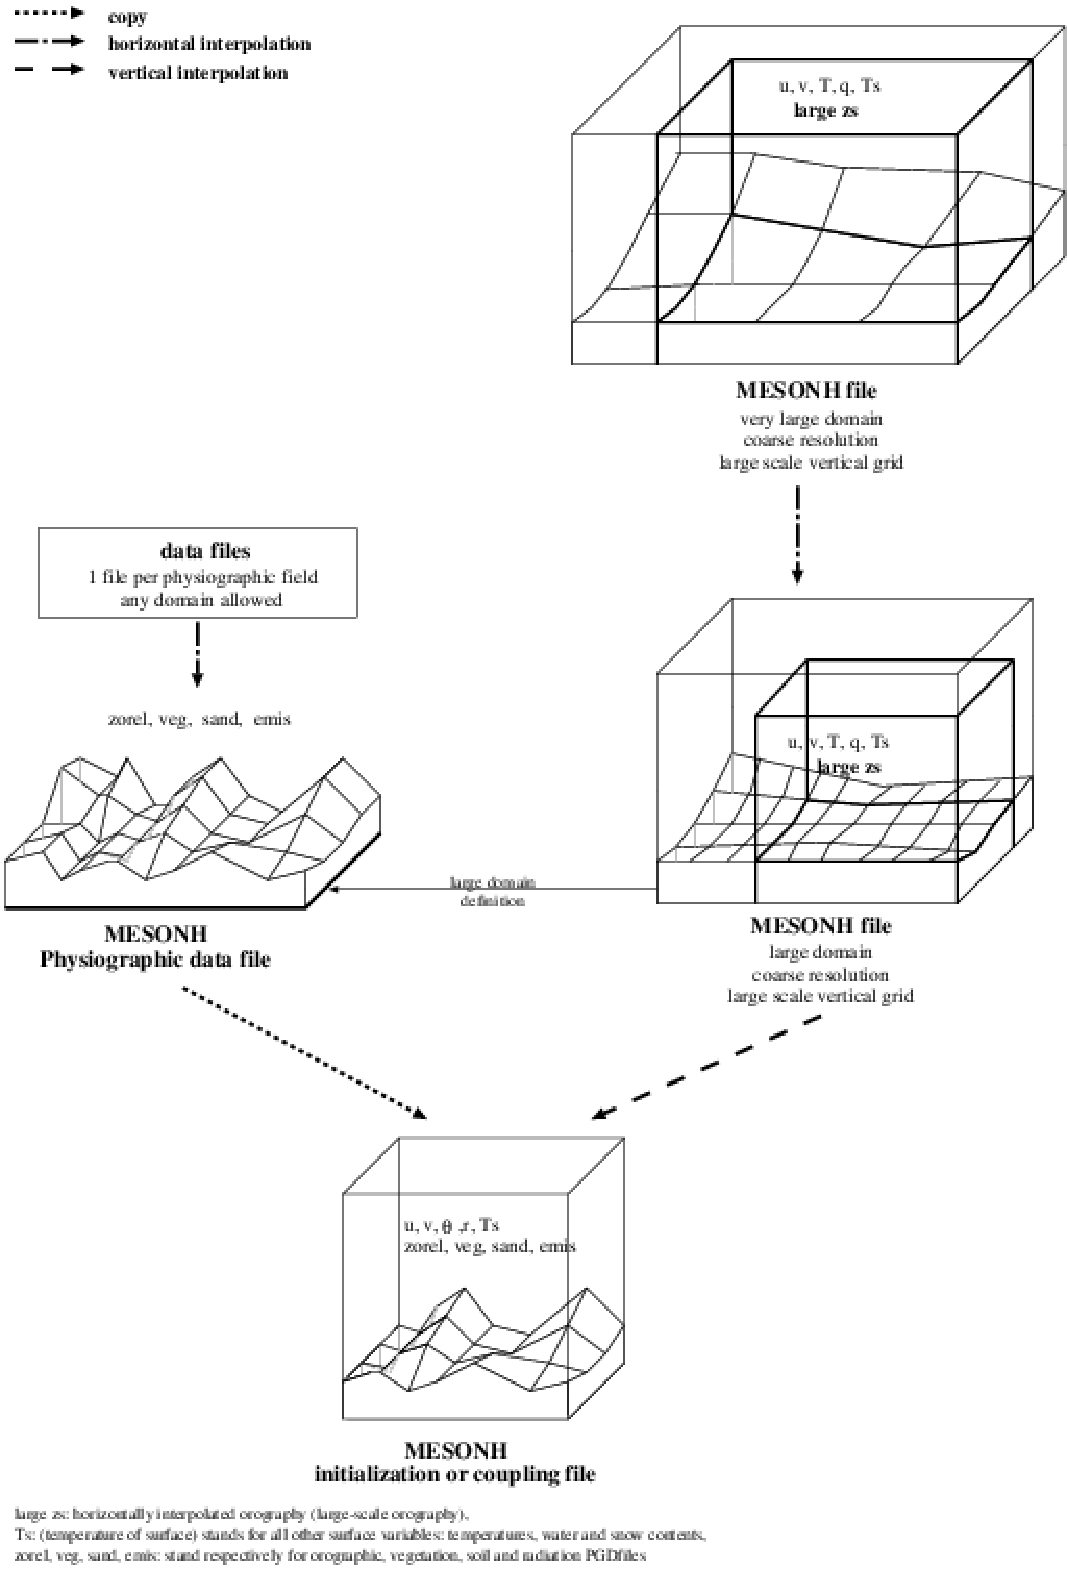
\includegraphics[width=14cm]{\EPSDIR/realcas_filiere_amont_spawning.pdf}}
\caption{schematic view of the interactions between the different files
during the initialization sequence of a real case simulation from a Meso-NH file.
\label{schematicsequence2}}
\end{figure}


\clearpage
%%%%%%%%%%%%%%%%%%%%%%%%%%%%%%%%%%%%%%%%%%%%%%%%%%%%%%%%%%%

\section{The PREP\_REAL\_CASE algorithm}

The Meso-NH program PREP\_REAL\_CASE performs the following tasks:
\begin{itemize}
\item the horizontal interpolation of the large-scale GRIB data fields
(in case of ALADIN, ARPEGE, or ECMWF archive).
\item the truncation of the horizontal domain (for convenience, one may want
to use very large horizontal domains for the large-scale files
(Aladin, Arpege, ECMWF or spawned\footnote{spawned file: file obtained after the
Meso-NH to Meso-NH horizontal interpolation program SPAWNING} Meso-NH files),
and run Meso-NH on a small fraction only (e.g. for testing).
\item the conversion, if necessary, of the prognostic variables of the input files to the
prognostic variables of Meso-NH (still on the input - or large scale - grid), and the
computation of the altitude of the points of this grid, in order to
prepare for the next steps.
\item the variables are subject to a special ``shifting'' process,
to take into account the difference between the large-scale and Meso-NH orographies.
\item Then the variables are vertically interpolated to the Meso-NH grid.
\item Finally, the wind and mass fields are forced to satisfy the
anelastic constraint, by one call to the pressure solver, and subsequent
modification of the fields.
\end{itemize}

The resulting Meso-NH file may be used to start a run. In practice,
sequences of such files are produced, separated by a few hours. The first
file is used to initialize the Meso-NH run, and subsequent files are
used to update the boundary conditions and/or the large-scale forcing
terms.

The remainder of the chapter describes those treatments in detail.

\section{Horizontal interpolation}

\subsection{Introduction}

The first step of PREP\_REAL\_CASE is the horizontal interpolation of the data fields
of the GRIB file (either ECMWF, ALADIN or ARPEGE archive) from the archive grid to the
chosen grid.\\

The following fields are interpolated :
\begin{itemize}
\item 3D fields
\begin{itemize}
\item wind component u
\item wind component v
\item absolute temperature T
\item specific humidity q
\end{itemize}
\item 2D ground and under surface fields
\begin{itemize}
\item soil surface temperature
\item sea surface temperature
\item deep ground temperature
\item surface water content
\item deep ground water content
\item snow
\end{itemize}
\end{itemize}

The next sections of the paragraph present the general interpolation scheme
and the specificity of each field.

\subsection{The interpolation algorithm}
The interpolations are performed on the 12 surrounding colocation points
(Fig. \ref{3Dhorinterp}), with a first interpolation along the latitudes
(with third order polynoms interpolation with 4 points and linear interpolation
for 2 points) and a second along the longitude (third order polynoms
interpolation):

\begin{figure}[!ht]
%\centerline{\includegraphics[width=10cm]{\EPSDIR/realcas_3Dhorinterp.eps}}
\centerline{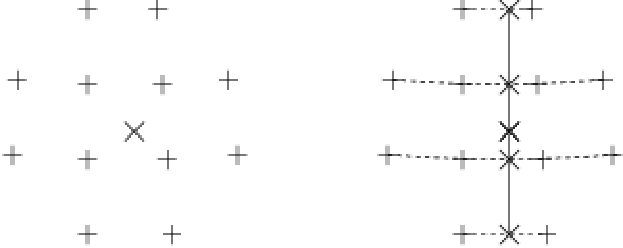
\includegraphics[width=10cm]{\EPSDIR/realcas_3Dhorinterp.pdf}}
\caption{Horizontal interpolations in FULL-POS.
\label{3Dhorinterp}}
\end{figure}

Masks may be used for surface fields. In this case, points are interpolated with
points of the same nature (mask value). For example, if we are interpolating a
point in the sea and we find that from the twelve surrounding points, only eleven
are sea points, the interpolation will take only these eleven points into account.
\\
For points which can not be correctly interpolated (points which are not surrounded
by enough data points of the same type), a special extrapolation is performed; the
given value is the one of the nearest data point of the same type.

\subsection{Definition of interpolated fields}
\begin{itemize}
\item Absolute temperature\\
From the archived absolute temperature is computed the virtual potential temperature
which is interpolated and then converted back to absolute temperature.\\
The used formula is the following one:\\
$\theta_v = T ( \frac{P}{P_0})^{-\frac{R_d}{C_pd}}
\; (1+\frac{R_v}{R_d}r_v)/(1+r_v)$

\item Specific humidity\\
The relative humidity is computed from the archived specific humidity and the archived
absolute temperature using the following formula:\\
$H=P\,q \, / ( \frac{R_d}{R_v}\epsilon_s(T) )$\\
$\epsilon_s(T)=\exp ( \alpha_w-\frac{\beta_w}{T}-\gamma_w\log(T) )$\\
H is interpolated and then the specific humidity is computed back.

\item Wind components u and v\\
The wind components are read separately and interpolated separately. The interpolation is
done on the value found in the archive, the definition vectors of u and v are projected
on Meso-NH coordinate system after the interpolation.\\
The projection of these vectors depends on the archive grid:
\begin{itemize}
\item ECMWF:\\
The grid used is a standard latitude, longitude one. The projection consists of a rotation
in the tangent plane. The rotation angle is given by the formula:\\
$\alpha=R_{pk}(\lambda-\lambda_0)-\beta$\\
where:\\
$R_{pk}$ is the projection coefficient of the Meso-NH domain,\\
$\lambda$ is the longitude of the point,\\
$\beta$ is the angle of rotation of the Meso-NH domain.
\item ARPEGE: \\
ARPEGE uses a stretched grid, therefore winds have first to be projected on a
 standard lat,lon grid (projection formulas were given by Meteo-France). The
projection is then processed in the same way as for ECMWF.
\item ALADIN: \\
Both Meso-NH and ALADIN use conformal projections, then the projection of the wind vector
consists of a rotation. The rotation angle is given by formula:\\
$\alpha=R_{pk}(\lambda-\lambda_0)-\beta - R_{pk_{ALADIN}}(\lambda-\lambda_{0_{ALADIN}})$
\end{itemize}
\item Soil temperature and sea temperature\\
The soil and sea temperature are computed from an interpolation of the surface temperature
using a land/sea mask.\\
To define if a data point from the archive is a land temperature or a sea temperature,
the archive land/sea mask is used. This land/sea mask is not a fraction of land, the
values store in the archives are integer. The output points are said to be from land
if the PGD land fraction is not null. They are said to be from sea if the PGD land
fraction is not equal to 1.\\
It should be noted that the mask defining the sea surface temperature and the one used
by the soil surface temperature are not complementary.
\item Deep ground temperature\\
The deep ground temperature is interpolated from the archived value, using the same mask
as for the soil temperature.
\item Soil and deep soil moisture\\
These fields are first converted from specific humidity to relative humidity, the
interpolation is performed and then they are converted back into specific humidity.\\
The value given are dependent of the soil model chosen for the archive. Therefore they
have to be converted to Meso-NH soil model.
\item Snow\\
Snow is interpolated using the same mask as for soil temperature.
\end{itemize}


%%%%%%%%%%%%%%%%%%%%%%%%%%%%%%%%%%%%%%%%%%%%%%%%%%%%%%%%%%%

\section{The different grids \label{prealgrid}}
Six grids are used in PREP\_REAL\_CASE: the first five share the same
location of the points on the horizontal, and the last one is a purely
vertical grid used for reference state computations (Fig.~\ref{fivegrids}).
\begin{itemize}
\item
{\bf{The large-scale grid}}: this grid is the one used either in the ALADIN file
or large-scale Meso-NH file. In the case of an ALADIN input file, this grid is
defined by the hybrid coordinate $\eta$, and has L levels. The position of
variables on this grid is shown in detail in Fig.~\ref{grids}. The
index of level on the large scale grid will be called $l$ hereafter.
\item
{\bf{The Meso-NH grid}}: this grid is the grid of the output Meso-NH file, which will be
used during the Meso-NH simulation for the 3D fields. It has (KE-KB+1)
physical levels (see Fig.~\ref{grids}), plus some levels under the ground or
at and over the model top ($z=H$) for boundary treatments.
This grid is defined by the Meso-NH orography and the vertical discretization
of the Gal-Chen coordinate $\widehat{z}$. The index of level will be called
$k$ hereafter.
\item
{\bf{The mixed grid}}: this grid is the Gal-Chen-Sommerville grid with
the same $\widehat{z}$ levels as the Meso-NH grid and the large scale
orography.
\item
{\bf{The shifted grid}}: this grid is the mixed grid on which has been applied
the shifting function (see hereafter). Therefore it follows the Meso-NH
orography, but it is not a Gal-Chen-Sommerville type grid.
It has the same number of levels as the Meso-NH grid, and the
levels are known by their altitudes.
\item
{\bf{The profile grid}}: this grid is the Gal-Chen-Sommerville grid with
the same $\widehat{z}$ levels as the Meso-NH grid and an orography defined
as the minimum of both orographies, $z_{min}$.
This grid allows to represent the free-atmosphere $\theta_v$ profiles
(see hereafter) whose value could be interpolated
on every point of both mixed and shifted grids. Note that $z_{min}$ can be
negative because of the spectral initial form of the large scale orography
(Gibbs phenomenon).
\item
{\bf{The reference grid}}: this grid is the Gal-Chen grid, a particular case of the
grid above, without orography. This grid is only used for the reference state.
\end{itemize}

For sake of clarity, the horizontal coordinates of the 3D fields are omitted
in the following equations.

\begin{figure}[!ht]
%\centerline{\includegraphics[width=16cm]{\EPSDIR/realcas_6grids.eps}}
\centerline{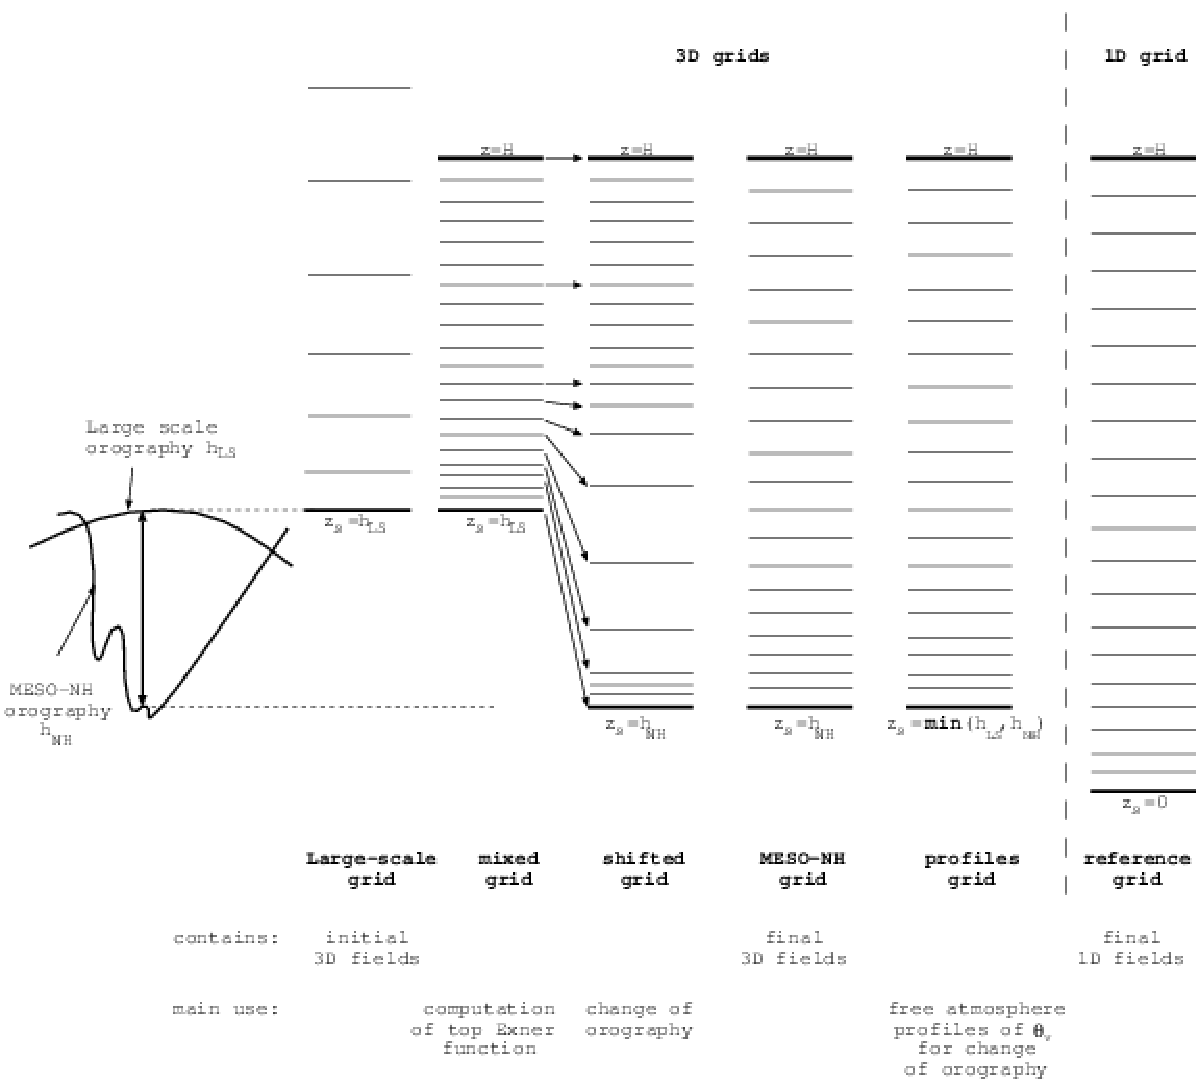
\includegraphics[width=16cm]{\EPSDIR/realcas_6grids.pdf}}
\caption{The six grids used in PREP\_REAL\_CASE, shown here for the case
where the Meso-NH orography is lower than the large-scale orography.
\label{fivegrids}}
\end{figure}

\clearpage

\begin{figure}[!ht]
%\centerline{\includegraphics[width=17cm]{\EPSDIR/realcas_grid.eps}}
\centerline{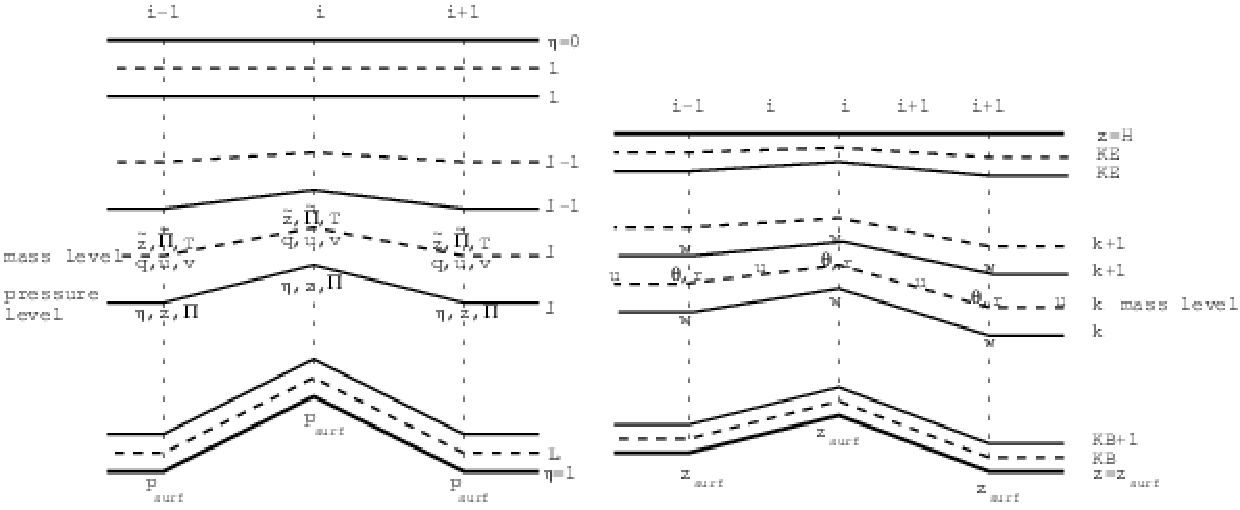
\includegraphics[width=17cm]{\EPSDIR/realcas_grid.pdf}}
\caption{ALADIN grid (left) and Meso-NH grid (right).
The main 3D-variables used or defined in this chapter
are shown, except v in the cross section of the Meso-NH grid because it
is located one half-mesh in front of the mass point.
\label{grids}}
\end{figure}
%%%%%%%%%%%%%%%%%%%%%%%%%%%%%%%%%%%%%%%%%%%%%%%%%%%%%%%%%%%
\section{Altitude of the ALADIN points and conversion of the variables}

This step is performed only when the input atmospheric large-scale file
is a GRIB one (if the input large-scale file is a Meso-NH one,
the variables are directly the correct ones). To preserve the largest
accuracy in the hydrostatic balance and the continuity equation through the
vertical interpolation process, we want to interpolate the quantities
$r_v$, $\theta_v$, $\rho u$, $\rho v$ and $w$. On the other hand, the GRIB
file contains the specific humidity $q$, the absolute temperature $T$,
and the wind components $u$ and $v$. All four variables are located on
the mass points of the ALADIN grid (Fig.~\ref{grids}),
therefore the altitudes of
those points must also be evaluated as accurately as possible. \\

{\bf Mixing ratio}

The mixing ratio of water vapor $r_v$ is readily obtained from the specific
humidity $q$ as
\begin{equation}
r_v=\left(\frac{1}{q}-1\right)^{-1}
\end{equation}

{\bf Virtual potential temperature}

The virtual temperature at the mass points of the ALADIN grid is readily obtained
as
\begin{equation}
T_v= T  (1+r_v R_v/R_d)/(1+r_v)
\end{equation}
To obtain the virtual potential temperature $\theta_v$, we must know the
Exner function $\Pi$ at the same levels.

Let us call $\tilde{\Pi}_l$ the
value of the Exner function at the mass level $l$ of the ALADIN grid, and
$\Pi_l$ the Exner function at the half levels of the same grid. The
latter is easy to compute because $P$ is known there:
\begin{equation}
\Pi_l= ({ P_l \over P_{00} })^{ R_d / C_{pd}}
\end{equation}
Then, we want to preserve the mass in each layer as accurately as possible
in the interpolation. We note that the discretization of the
hydrostatic relation in the ALADIN file would read with the alternative
variables $T_v$ and $\theta_v$
\begin{eqnarray}
\label{pi1}
z_l-z_{l-1}=&-\frac{C_{pd}T_{v_l}}{g}&(\ln\Pi_l-\ln\Pi_{l-1})\\
\label{pi2}
z_l-z_{l-1}=&-\frac{C_{pd}\theta_{v_l}}{g}&(\Pi_l-\Pi_{l-1})
\end{eqnarray}
This leads to the optimal way of computing
\begin{equation}
\tilde\Pi_l=\frac{\Pi_l-\Pi_{l-1}}{\ln\Pi_l-\ln\Pi_{l-1}}
\end{equation}
from which the virtual potential temperature follows
\begin{equation}
\theta_{v_l} = T_{v_l} / \tilde{\Pi}_l
\end{equation}

{\bf Altitude of the points of the large-scale grid}

Since all variables are located at the mass points of the ALADIN grid,
in order to perform the vertical interpolation, one must compute the
altitudes of these points.

1) The altitude of each pressure point is given by integration
of the hydrostatic relation from bottom to top, discretized as equation
(\ref{pi2}).

2) Assuming a linear variation of $\theta_v$ with $\eta$,
the altitude $\tilde{z_l}$
of the mass point on level l is given by:
\begin{equation}
\tilde{z_l}=z_l-\frac{C_{pd}\left( \frac{3}{4}\theta_{v_l}
+\frac{1}{4}\theta_{v_{l+1}}\right)}{g}(\tilde\Pi_l-\Pi_l)
\end{equation}

{\bf Horiozontal wind components}

The wind components are initially contravariant on the ALADIN grid
(i.e. following the iso-$\eta$ surfaces and not true horizontal planes).
They are projected onto each true horizontal plane containing the considered
point.\\

{\bf Vertical wind components}

It is retrieved from the approximated formula of diagnostic vertical velocity
in models with $\eta$ coordinate. If $\eta$ equal 0 at model top
and 1 at ground, and with  $p=A(\eta)p_{0}+B(\eta)p_{s}$:
\begin{eqnarray}
gw & = & \frac{1}{\rho}\int^\eta_0\vec{\nabla}_\eta
\l (\frac{dA}{d\eta '}p_0+\frac{dB}{d\eta '}p_{s})\vec{U}\r d\eta ' \nonumber \\
& & -\frac{B(\eta)}{\rho}\int^1_0\vec{\nabla}_\eta
\l(\frac{dA}{d\eta '}p_0+\frac{dB}{d\eta '}p_{s})\vec{U}\r d\eta ' 
+\frac{\rho_{s}}{\rho}B(\eta)\vec{U}\cdot \vec{\nabla}(g\, z_{s}) \nonumber
\end{eqnarray}

\section{Interpolation to the mixed grid}

The fields are interpolated to the mixed grid (there is no
change of orography).
Then, if the chosen vertical grid top is higher than the highest
input model one,
the program aborts. There is no extrapolation, and therefore, the
new vertical grid must not go too high.

{\bf Pressure at the model top}

The values of $\Pi$ at the altitude $z=H$ (top of the Meso-NH grid) are
determined by vertical integration of the hydrostatic equation from bottom
to top (surface pressure is known).
This integration is performed on the mixed grid, where all
variables have been interpolated, because its discretization
will be approximately the same as the Meso-NH grid (only change of orography).
If computed with the ALADIN grid, even with attention paid to mass
conservation, one could have for ALADIN levels spaced more than 3~km apart
an error of 1~hPa on the surface pressure, when reintegrated with the Meso-NH
grid. This error is evident at the model top.

The field of Exner function at model top is hereafter noted
$\Pi^{top}(x,y)$.  It will be used to compute the total dry mass.\\


{\bf Horizontal momentum}

We compute $\rho$ on the mass points of the mixed grid as:

\begin{equation}
\label{eq:rhod}
{\rho_d}=\frac{P_{00}(\Pi)^{C_{pd}/R_d -1}}
{R_d\theta_v}
\end{equation}

The values of $\rho u$ and $\rho v$ follow.

\section{The shifting process}

The next step is to account for the differences in the ALADIN and Meso-NH
orographies. There is no standard way of doing this, and the treatment
relies on conceptual ideas on the way the flow reacts to the presence of
the orography. We also want to preserve some information on the boundary
layer structure, inasmuch as possible.

The basic conceptual model is that the whole atmosphere will be vertically
displaced (shifted) from the large-scale orography to the Meso-NH orography
(Fig.~\ref{physhift}). The maximum vertical
displacement occurs at the ground, where it equals $h_{NH}-h_{LS}$. Further
aloft, the displacement diminishes, and is negligible at some height
$z_{scale}$ above the ground. So, we define the shifting function
\begin{equation}
\label{shift}
f(z)=z+(h_{NH}-h_{LS})\left( 1-\mbox{tanh}^2
\left(\frac{z-h_{LS}}{z_{scale}}\right)\right)
\end{equation}
as the vertical displacement experienced by a parcel located at altitude
$z$ on the large-scale grid.
By default, $z_{scale}$ takes the value of 1000~m.\\

The next problem is to choose those quantities which will be conserved
during the shifting process. This clearly has important consequences: for
instance, if $r_v$ and $\theta_v$ were conserved, this would generate
warm and dry anomalies in the valleys resolved by the Meso-NH orography,
and unresolved by the large-scale orography. This is not desirable.

\clearpage


\begin{figure}[!ht]
%\centerline{\includegraphics[width=16cm]{\EPSDIR/realcas_physhift.eps}}
\centerline{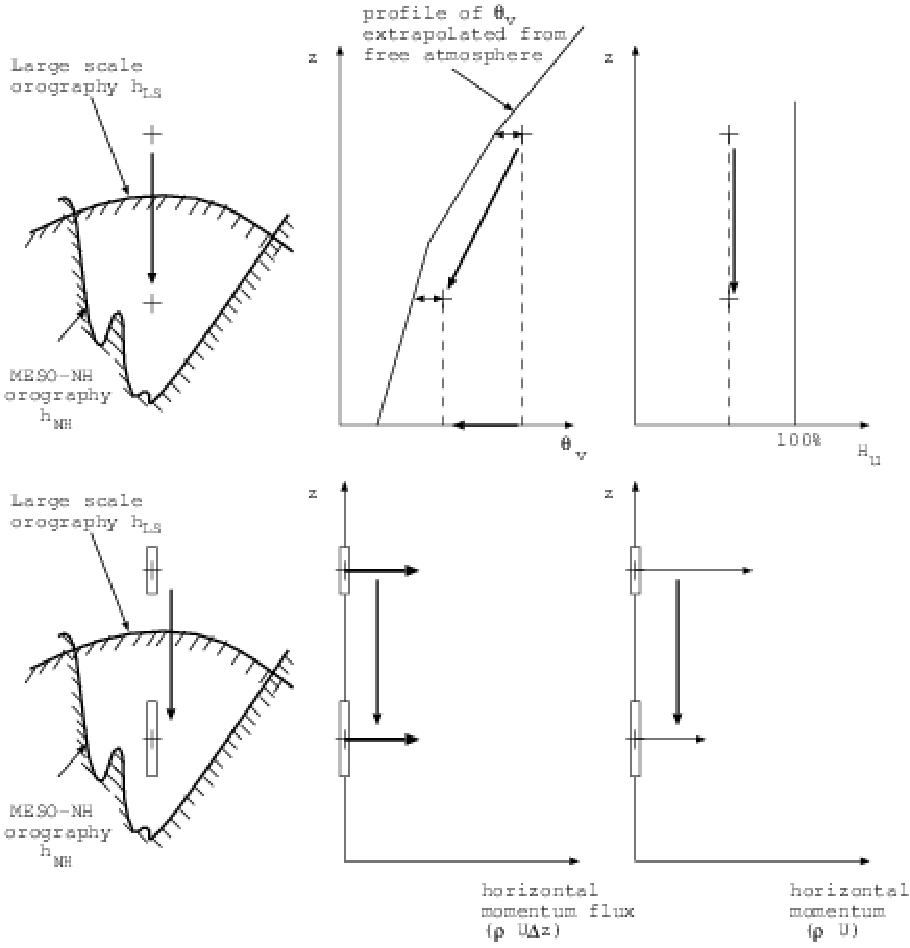
\includegraphics[width=16cm]{\EPSDIR/realcas_physhift.pdf}}
\caption{Action of the shift on the variables for one point shifted down
\label{physhift}}
\end{figure}

\clearpage

The current version of the program conserves
\begin{itemize}
\item
the difference between $\theta_v$ (virtual potential temperature)
and $\theta_v$ 'free atmosphere profile'.
This profile is the one where the boundary layer has been removed.
It is constructed in the following
manner, which has been found to work fairly well from polar to Saharian
boundary layers:
\begin{enumerate}
\item the boundary layer top is found with an algorithm checking
$\partial \theta_v / \partial z$, and comparing it to
the gradient between 5000~m of height and the ground.
\item the $\theta_v$ values under this boundary layer top are replaced
considering a constant gradient equal to the one between 5000~m of height
and the boundary layer top.
\end{enumerate}
\item
the relative humidity $H_u=100 * p/e_s(T)/(R_d/R_v/r_v + 1)$
\item
The difference between pressure and hydrostatic pressure.
This quantity is zero per definition when input file is an ALADIN one, but
is non-zero for a Meso-NH one. This allows to interpolate in some
extent the non-hydrostatic effects.
\item
the horizontal mass flux $\rho J u, \rho J v$
in the corresponding grid layer. $J$ is the Jacobian, or volume of the grid
box. In practice, since the horizontal grid size is the same for the two
grids, it is sufficient to conserve the product of $\rho u$ and $\rho v$
by the vertical grid size.
\item
the vertical velocity $w$. However, it is modified in the upper quarter
of atmosphere to obtain a zero value at model top.
This will not produce a correct value near the ground (because of new orography).
The aim of this is to construct a smooth vertical velocity field for
$w_{LS}$. The initial field $w$ will be produced from this
guess by the pressure solver.
\end{itemize}

Therefore there is usually cooling, moistening, and wind speed decrease
if the point is shifted down (in a valley, see Fig.~\ref{physhift}),
and warming, drying and wind speed increase if the point is shifted up
(above a peak or ridge).

\section{Vertical interpolation}

The next step is to perform the vertical interpolation from the
shifted grid to the Meso-NH grid. Since the two grids share the same
definition of the orography, this is relatively straightforward.
Llinear interpolation is used.

The variables subject to interpolation are $\theta_v$, $H_u$, $\rho u$,
$\rho v$, $w$ and the difference between pressure and hydrostatic pressure.
They are interpolated to the mass points of the Meso-NH grid.
Hydrostatism is recomputed from model top, and pressure is deduced afterwards.

Then, $r_v$ is recovered iteratively from $\theta_v$ and $H_u$, and $\theta$
from $\theta_v$ and $r_v$ by:
\begin{equation}
\theta=\theta_v\frac{1+r_v}{1+\frac{R_v}{R_d}r_v}
\end{equation}

Finally, the wind components on the Arakawa C-grid are written as
\begin{eqnarray}
(\rho u)=\overline{(\rho u)}^x \\
(\rho v)=\overline{(\rho v)}^y
\end{eqnarray}
The fields are now correctly localized on the final Meso-NH grid.

\section{Reference state}

The reference state is computed on the reference grid, as the horizontal
average of the actual state.

First, $\theta_{v\,ref}$ and $r_{v\,ref}$ are computed as a mean value at
constant altitude of the $\theta_v$ and $r_v$ field, after interpolation
to the reference grid.

$\Pi_{ref}^{top}$ is computed as the horizontal average of $\Pi^{top}(x,y)$.
Then, the hydrostatic relation for the reference state
is integrated from top to bottom to compute $\Pi_{ref}$.
\begin{equation}
d\Pi_{ref}=-\frac{g}{C_{pd}\theta_{v\,ref}}dz
\end{equation}
Finally, the density of dry air for the reference state is retrieved
\begin{equation}
\rho_{d\,ref}=\frac{P_{00}(\Pi_{ref})^{R_d/C_{pd}-1}}
{R_d \theta_{v\,ref}(1+r_{v\,ref})}
\end{equation}

\section{Computation of the total dry air mass}
The total dry air mass within the domain of integration of the model
is needed to resolve accurately the pressure problem (see Chapter 2).
First, $\Pi$ is computed by integration of the exact hydrostatic relation
\begin{equation}
d\Pi=-\frac{g}{C_{pd}\theta_v}dz
\end{equation}
from the top ($\Pi^{top}(x,y)$) to the bottom of the integration domain.
Then, $\rho_d$ is computed as
\begin{equation}
\label{eq:rhodd}
{\rho_d}=\frac{P_{00}(\Pi)^{R_d/C_{pd}-1}}
{R_d\theta_v(1+r_v)}
\end{equation}
The total dry mass is deduced
\begin{equation}
{\cal{M}}_d=\int\int\int_V\rho_ddV
\end{equation}

\section{Anelastic constraint}

The final step is to enforce the anelastic constraint.
The first guess velocity field $\vec{U}_{fg}$ = ($u$, $v$, $w$) does not verify the lower
boundary condition. It also does not satisfy the anelastic
constraint, with the reference dry air density. Those two deficiencies are
corrected by use of the subroutine ANEL\_BALANCE (see previous
chapter for a description). The input field for this routine is
$\rho_d \vec{U}_{fg}$, and the output field, $\rho_{d\,ref} \vec{U}$,
satisfies all necessary constraints to start an integration.


%
%%%%%%%%%%%%%%%%%%%%%%%%%%%%%%%%%%%%%%%%%%%%%%%%%%%%%%%%%%%%%%%%%%%%%%%%%%%%%%
%%%%%%%%%%%%%%%%%%%%%%%%%%%%%%%%%%%  END OF REAL CASE %%%%%%%%%%%%%%%%%%%%%%%%
%%%%%%%%%%%%%%%%%%%%%%%%%%%%%%%%%%%%%%%%%%%%%%%%%%%%%%%%%%%%%%%%%%%%%%%%%%%%%%
%
